\documentclass[a4paper,11pt,bibliography=totoc, listof=totoc,titlepage]{scrartcl}
\usepackage[ngerman]{babel}
\usepackage[utf8]{inputenc}
\usepackage[left=3cm,right=2.5cm,top=2.5cm,bottom=2.5cm]{geometry}
\usepackage[onehalfspacing]{setspace}
\renewcommand{\arraystretch}{1.5}
\usepackage{graphicx}
\usepackage{color}
\usepackage[usenames,dvipsnames,table,xcdraw]{xcolor}
\usepackage[toc,page]{appendix}
%\usepackage[scaled]{berasans}
%\renewcommand*\familydefault{\sfdefault}  %% Only if the base font of the document is to be sans serif
%\usepackage[T1]{fontenc}

  
\usepackage[hyphens]{url}
\usepackage[hidelinks]{hyperref}
\usepackage{todonotes}
\usepackage{amsmath}

\usepackage{multirow}

\newcommand*\justify{%
  \fontdimen2\font=0.4em% interword space
  \fontdimen3\font=0.2em% interword stretch
  \fontdimen4\font=0.1em% interword shrink
  \fontdimen7\font=0.1em% extra space
  \hyphenchar\font=`\-% allowing hyphenation
}

\newcommand{\code}[1]{\texttt{\justify{#1}}}
%\usepackage{tocloft}

%Boxfehler
\hbadness=1000000

% Listings
\usepackage{listings}
\lstset{
   breaklines=true,
   captionpos=t,
   basicstyle=\scriptsize\ttfamily,
   keywordstyle=\bfseries\ttfamily\color{orange},
   stringstyle=\color{green}\ttfamily,
   commentstyle=\color{gray}\ttfamily,
   emph={square}, 
   emphstyle=\color{blue}\texttt,
   emph={[2]root,base},
   emphstyle={[2]\color{yac}\texttt},
   showstringspaces=false,
   flexiblecolumns=false,
   tabsize=2,
   numbers=left,
   numberstyle=\tiny,
   numberblanklines=false,
   stepnumber=1,
   numbersep=10pt,
   xleftmargin=15pt
 }

% Zitierstil
%\usepackage[style=authoryear,citestyle=authoryear,natbib=true]{biblatex}
%\bibliography{Thesis.bib}
\usepackage[round]{natbib}
%\bibliographystyle{hcu}


\usepackage[toc]{glossaries}
\makeglossaries

\newglossaryentry{Suchfenster}
{
    name=Suchfenster,
    description={Dieses Auswahlmenü unterstützt die Suche in den Klartexten. Hierbei kann auch nach Teilen gesucht werden. Bei Eingabe von ``rad'' würde nicht nur der ``Fahrradweg'' gefunden werden sondern auch der ``Mehrzweckstreifen mit Fahrradbenutzung''}
}
\newglossaryentry{Querschnitt}
{
    name=Querschnitt,
    description={Ein Querschnitt ist eine Fläche eines Querschnittes.}
}

\begin{document}
\pagenumbering{Roman}
\begin{titlepage}
\begin{center}
\renewcommand{\arraystretch}{0.7}
\begin{tabular}{lr}
\begin{tabular}{l}
\end{tabular} \hspace{0.5cm} &
\begin{tabular}{r}
Landesbetrieb Geoinformation und Vermessung\\
Neuenfelder Straße 19\\
21109 Hamburg\\
\end{tabular}
\end{tabular}\\\vspace{5cm}
\doublespacing 
{\huge\bfseries  QuerschnittsEditor
}\vspace{0.5cm}\\

{\large\bfseries Bedienerhandbuch
}\vspace{2cm}\\
{\large Florian Timm}\\

\vspace{10cm}
Stand: 17. Feb. 2020\\
\end{center}
\setcounter{page}{0} 
\end{titlepage}


% Mehrere gleichzeitig zitieren
\providecommand{\citeTwo}[4]{\citep[{\citealp[#1]{#2};}][#3]{#4}} 
\providecommand{\citeThree}[6]{\citep[{\citealp[#1]{#2}; \citealp[#3]{#4};}][#5]{#6}} 
\providecommand{\citeFour}[8]{\citep[{\citealp[#1]{#2}; \citealp[#3]{#4}; \citealp[#5]{#6};}][#7]{#8}}

\newpage

\tableofcontents
\newpage

\pagenumbering{arabic}
\setcounter{page}{1} 

\section{Grundlagen}
Der LGV-QuerschnittsEditor dient zur Bearbeitung von \Gls{Querschnitt}en, Verkehrszeichen und punktueller Straßenausstattung in der TTSIB. Er ermöglicht eine graphische Stationierung von Elementen, ohne das hierbei manuell Stationierungen festgelegt werden müssen.

\subsection{Login}
\begin{figure}
 \centering
 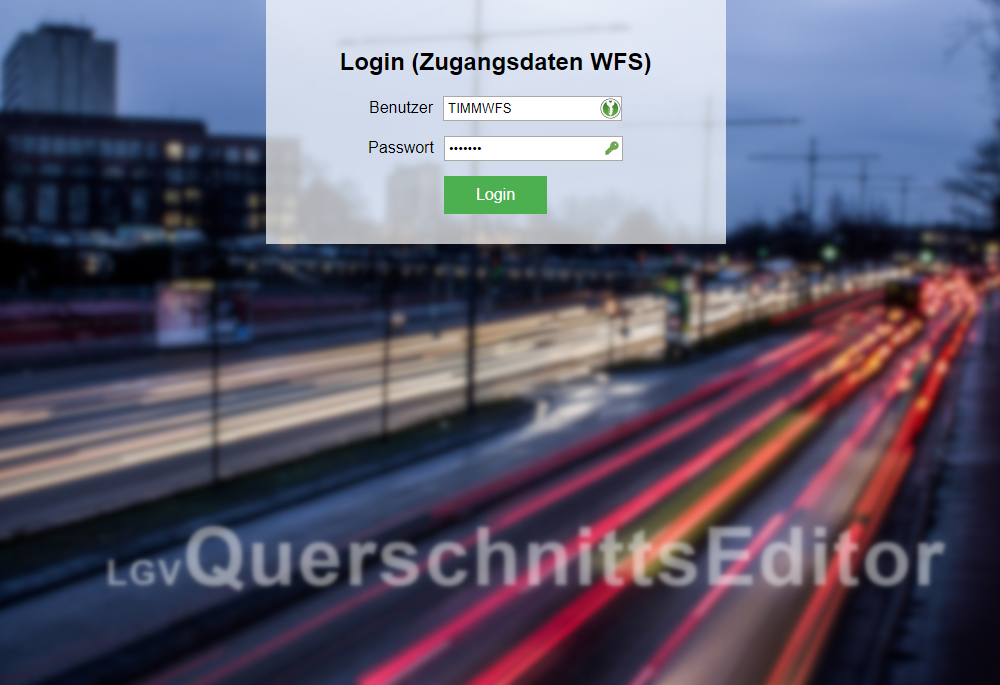
\includegraphics[width=.8\textwidth]{./img/login.png}
 \caption{Login-Oberfläche}
 \label{img:login}
\end{figure}

\label{ss:login}
Der Login (\autoref{img:login}) erfolgt mit Zugangsdaten des PublicWFS. Diese Zugangsdaten können, müssen aber nicht identisch sein mit den Zugangsdaten zu der TTSIB/INFOSYS und sind einzeln im Administratortool des PublicWFS anzulegen. 



\subsection{Auswahl des Ereignisraumes}

\begin{figure}
 \centering
 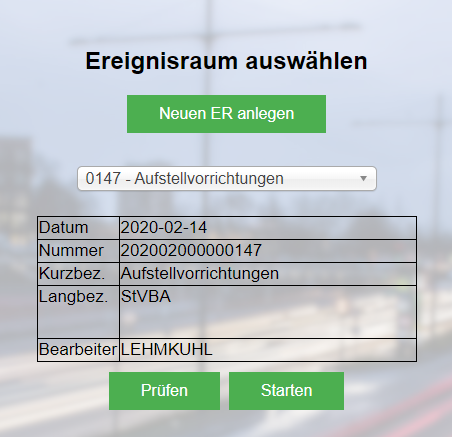
\includegraphics[width=.7\textwidth]{./img/er_auswahl.png}
 \caption{Auswahl des Ereignisraumes}
 \label{img:er_auswahl}
\end{figure}

Nach dem Login (siehe \autoref{ss:login}) öffnet sich die Auswahl des Ereignisraumes (\autoref{img:er_auswahl}). Hier ist es möglich bestehende Datenereignisräume auszuwählen, zu prüfen oder neue anzulegen. Durch Auswahl eines Ereignisraumes (ER) in der Drop-Down-Liste werden in der Tabelle hierunter die Informationen zu dem ausgewählten ER angezeigt. Durch einen Klick auf Starten wird der Ereignisraum über den PublicWFS geladen und die Objekte, die sich in dem Ereignisraum befinden geladen.



\subsection{Bearbeitungsmodus}
\begin{figure}
 \centering
 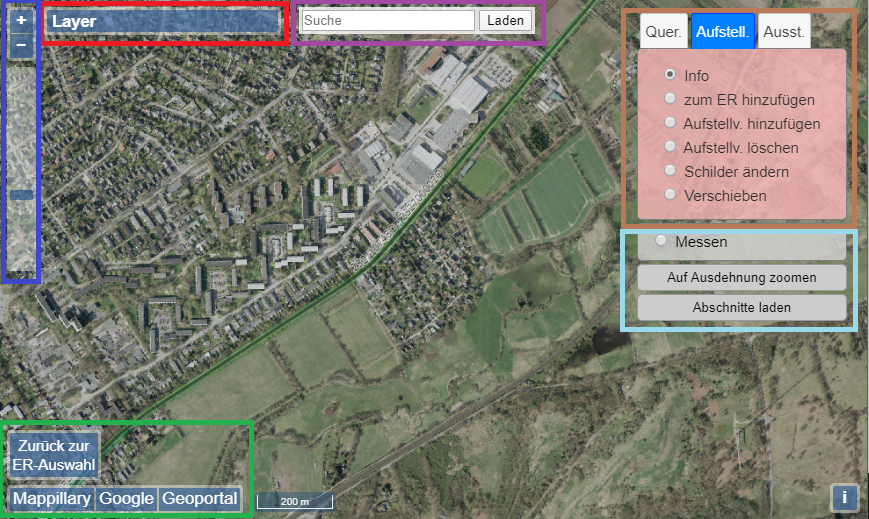
\includegraphics[width=.9\textwidth]{./img/bearbeitung.png}
 \caption{Bearbeitungsmodus}
 \label{img:bearbeitung}
\end{figure}
Wenn der Ereignisraum fertig geladen wurde, ist die Bearbeitung von Objekten möglich (\autoref{img:bearbeitung}). Wenn der Ereignisraum bereits Daten enthält, werden Straßenabschnitte und die Objekte angezeigt und auf diese gezoomt. Wenn keine Daten im Ereignisraum vorhanden sind, wird eine leere Karte angezeigt und eine Meldung angezeigt, dass keine Daten vorhanden sind.



\subsubsection{Kartensteuerung}
Die Karte wird mit der Maus gesteuert. Durch Klicken und Halten der linken Maustaste wird die Karte verschoben.Hineingezoomt werden kann mit einem Doppelklick oder mit dem Plus oben links (dunkelblauer Kasten). Herausgezoomt wird mit dem Minus-Zeichen hierdrunter. Außerdem lässt sich die Karte mit dem Mausrad vergrößern oder verkleinern sowie mit dem Schieberegler am linken Bildrand (dunkelblauer Kasten auf \autoref{img:bearbeitung}). Eine Orientierung der Zoomstufe bietet der Maßstabsbalken am unteren Bildrand.

Mit den mittleren Schaltfläche im hellblauen Kasten wird auf die geladenen Objekte gezoomt. 

\begin{figure}
 \centering
 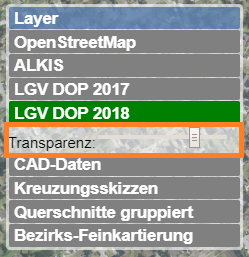
\includegraphics[width=.4\textwidth]{./img/layerbaum.png}
 \caption{Layerbaum}
 \label{img:layerbaum}
\end{figure}

\paragraph{Layerbaum} Mit der Schaltfläche Layer im roten Kasten auf \autoref{img:bearbeitung} können die Hintergrundkarten umgeschaltet werden. Beim Überfahren der Schaltfläche mit der Maus öffnet sich der Layerbaum (\autoref{img:layerbaum}). Durch Klick auf die grauen Schaltflächen wird der Layer aktiviert, mit Klick auf eine grüne Schaltfläche wird der Layer wieder deaktiviert. Außerdem besteht die Möglichkeit, die Transparenz einzelner Layer anzupassen (oranger Kasten). 

\subsubsection{Abschnitte laden}
\label{ss:abschnitteladen}
\paragraph{Abschnitte laden nach Kartenausschnitt}
Die Schaltfläche Abschnitte laden (hellblauer Kasten) lädt alle Straßenabschnitte, die sich im Kartenausschnitt befinden (jedoch maximal 1000) aus der TTSIB.

\paragraph{Suche}
Mit der Suche im violetten Kasten in \autoref{img:bearbeitung} kann nach Straßen gesucht werden. Die Suche ist möglich über Wegenummern, Netzknoten und Straßennamen. Nach dem Klick auf Laden werden die zutreffenden Abschnitte geladen und auf diese gezoomt.

\subsubsection{Bearbeitungswerkzeuge}
Mit dem Schaltflächen im braunen Kasten werden die Bearbeitungswerkzeuge gesteuert. Diese werden in einzelnen Abschnitten erläutert.

\begin{itemize}
    \item \Gls{Querschnitt}e in \autoref{s:querschnitte}
    \item Aufstellvorrichtungen und Verkehrszeichen in \autoref{s:schilder}
    \item Straßenausstattung in \autoref{s:straus}
\end{itemize}

\subsubsection{Weitere Tools}
\paragraph{Messen}
Mit der Schaltfläche \verb|Messen| lässt sich ein Messwerkzeug aktivieren. Mittels einfachen Klick in die Karte können Stützpunkte gesetzt werden, mittel Doppelklick wird die Messung beendet. Beim Wechsel des Werkzeuges oder beim Beginn einer neuen Messung wird die alte Messung gelöscht.

\paragraph{Andere Kartendienste}
Mit den Schaltflächen unten links (grüner Kasten) kann zu anderen Kartenportalen gesprungen werden. Hierbei wird das Kartenzentrum und der Maßstab annährend beibehalten. Die Seite wird in einem neuen Browser-Tab geöffnet. Bei einem weiteren Klick wird dieser Browser-Tab aktualisiert.

\section{Querschnitte bearbeiten}
\label{s:querschnitte}

Zwischen den einzelnen Objektarten-Modi kann mit den Tabs auf der rechten Seite umgeschaltet werden. Durch Klick auf \verb|Quer.| wird die Bearbeitung von \Gls{Querschnitt}en ermöglicht.

\subsection{Querschnitte laden}
Sofern von Abschnitten nicht schon eine andere Objektklasse im Editor im Ereignisraum liegt, muss der gewünschte Abschnitt erst einmal in das Programm geladen werden. Hierfür kann die Suche oder der Button Abschnitte laden verwendet werden (siehe \autoref{ss:abschnitteladen}). Nach dem Klick auf \verb|zum ER hinzufügen| kann der Abschnitt durch Klick auf diesen in der Karte dem Ereignisraum hinzugefügt werden.

Der Abschnitt wird nun in den Ereignisraum geladen, die Daten aus der TTSIB übertragen und in der Karte die bestehenden \Gls{Querschnitt}e des Abschnittes angezeigt.

\subsection{Querschnitte hinzufügen}
Fehlende \Gls{Querschnitt}sflächen können mit dem Tool \verb|Fläche hinzufügen| hinzugefügt werden. Nachdem Aktivieren des Tools kann eine Trennlinie oder die Bestandsachse ausgewählt werden. Rechts unten werden nochmals Informationen zu dem ausgewählten \Gls{Querschnitt} angezeigt. Die neue Fläche wird auf der der Bestandsachse abgewandten Seite der ausgewählten \Gls{Querschnitt}sfläche hinzugefügt (also an der Stelle, an der die Trennlinie gewählt wurde). Durch Klick auf \verb|Querschnitt hinzufügen| wird die Fläche erzeugt. Falls die Bestandsachse gewählte wurde, folgt nach dem Klick auf \verb|Querschnitt hinzufügen| ein Dialog, in dem abgefragt wird, auf welcher Seite der Mittelachse der Streifen angefügt werden soll. In allen Fällen wird eine neue Fläche mit den Eigenschaften des ausgewählten Streifen und einer Breite von 275~cm hinzugefügt. Diese muss dann mit dem Tool \verb|Fläche ändern| (siehe \autoref{ss:flaecheaendern}) verändert werden -- vor allem falls eine Bestandsachse angefügt wurde, da hiervon nur eine existieren darf.

\subsection{Attribute ändern}
\label{ss:flaecheaendern}
Attribute von \Gls{Querschnitt}sflächen können mit dem Tool \verb|Fläche ändern| angepasst werden. Das Tool unterstützt die Änderungen von einzelnen und mehreren Flächen.

\paragraph{Einzeländerung}
\label{p:flaecheeinzeln}
Um eine Fläche einzeln zu bearbeiten, kann diese einfach in der Karte per Klick ausgewählt werden. Im rechten Rand werden nun die Informationen der Fläche angezeigt. Die Eigenschaften Art und Art der Oberfläche lassen sich mit \Gls{Suchfenster}n auswählen und ändern. Die Breite der Fläche kann per Zahleneingabe in Zentimetern angepasst werden. Alle Änderungen in diesem Menü müssen mit \verb|Speichern| übernommen werden. Ansonsten werden bei der Auswahl einer anderen Fläche oder beim Umschalten des Werkzeuges die neuen Eigenschaften verworfen.

\paragraph{Mehrfachänderung}
Das Werkzeug unterstützt auch die Änderung mehrerer Flächen mit einmal hierfür muss die \verb|Strg|-Taste auf der Tastatur gedrückt werden, während die zu ändern\-den Flächen mit der Maus ausgewählt werden.

Im rechten Rand wird nun die Art und die Art der Oberfläche der gewählten Flächen sowie deren Anzahl angezeigt. Sofern sich die Attribute der einzelnen Flächen unterscheiden, wird im entsprechenden Feld ``- verschiedene -'' angezeigt. Durch Auswahl eines anderen Wertes in den beiden \Gls{Suchfenster}n, wird das geänderte Attribut für alle ausgewählten Abschnitte gesetzt.

\subsection{Flächen anpassen}
Neben der Bearbeitung von Flächen durch Eingabe von Breiten in der Attributtabelle (siehe \autoref{p:flaecheeinzeln}) ist es auch möglich, diese in der Karte zu verändern. Auch hierfür dient das Werkzeug \verb|Fläche ändern|. Durch Auswahl einer Querschnittsfläche erscheinen auf der der Achse abgewandten Trennlinie ein roter und ein grüner Punkt. An diesen Punkten kann mittels Klicken und Ziehen die Breite verändert werden. Die Punkte können nur auf der schwarzen Linie der von- oder bis-Station verschoben werden. Während des Verschiebens erscheint eine Vorschau der neuen Trennlinie. Beim Loslassen des Punktes wird die veränderte Fläche gespeichert.

Mit den Schaltflächen unter der Attributtabelle lassen sich Einstellungen der Manipulation der Flächen anpassen. Mit den Radioknöpfen \verb|...verschieben| und \verb|...anpassen| verändert sich das Verhalten der weiter außen liegenden Querschnitte. Bei der Manipulation werden diese je nach gewählter Einstellung verschoben oder in ihrer Breite so verändert, dass die Änderung der manipulierten Fläche ausgeglichen wird.

Mit dem Kontrollkästchen \verb|angrenzende Querschnitte mitziehen| wird dafür gesorgt, dass der auf der anderen Seite der Querschnittsstation liegende Querschnitt mit angepasst wird.

\subsection{Flächen teilen}
Die Funktion ``Querschnitt teilen'' ermöglicht es, Querschnittsflächen in ihrer Längsrichtung zu teilen. Nach Aktivierung des Werkzeuges erscheint beim Überfahren des Abschnittes mit der Maus eine Vorschau der Trennlinie. Durch Klicken kann diese fixiert werden. Die Teilung findet dann nach einem Klick auf Teilen in der rechten Bildschirmleiste statt.


\subsection{Flächen löschen}
Um Flächen zu Löschen muss nach dem Aktivieren des Werkzeuges die zu löschende Fläche ausgewählt werden. Am rechten Rand erscheint dann eine rote Schaltfläche zum Löschen der ausgewählten Fläche.

\section{Aufstellvorrichtungen und Verkehrszeichen bearbeiten}
\label{s:schilder}
Zwischen den einzelnen Objektarten-Modi kann mit den Tabs auf der rechten Seite umgeschaltet werden. Durch Klick auf \verb|Aufstell.| wird die Bearbeitung von Aufstellvorrichtungen und Verkehrszeichen ermöglicht.

\subsection{Aufstellvorrichtungen laden}
Sofern von Abschnitten nicht schon eine andere Objektklasse im Editor im Ereignisraum liegt, muss der gewünschte Abschnitt erst einmal in das Programm geladen werden. Hierfür kann die Suche oder der Button Abschnitte laden verwendet werden (siehe \autoref{ss:abschnitteladen}). Nach dem Klick auf \verb|zum ER hinzufügen| kann der Abschnitt durch Klick auf diesen in der Karte dem Ereignisraum hinzugefügt werden.

Der Abschnitt wird nun in den Ereignisraum geladen und die an ihm liegenden Aufstellvorrichtungen geladen.

\subsection{Aufstellvorrichtungen hinzufügen}
Mit dem Werkzeug \verb|Aufstellv. hinzufügen| können neue Aufstellvorrichtungen erzeugt werden. Es erscheint nach der Aktivierung eine blaue Stationierungslinie. Mit dieser ist es möglich, die gewünschte Position der neuen Aufstellvorrichtung festzulegen. Sie rastet automatisch auf den möglichen Stationierungen ein. Es kann bei Bedarf mit einem Klick auf einen Abschnitt festgelegt werden, dass nur auf diesem Abschnitt stationiert werden soll.

Rechts am Bildschirmrand lassen sich die Attribute der neu anzulegenden Aufstellvorrichtung einstellen und anschließend mit einem Klick auf \verb|Hinzufügen| speichern. Nun wird die neue Aufstellvorrichtung gespeichert.

\subsection{Aufstellvorrichtung verändern}
Mit dem Tool \verb|Verschieben| lassen sich Attribute ändern und Aufstellvorrichtungen verschieben. 

\paragraph{Verschieben} 
Hierfür wird die zu ändernde Aufstellvorrichtung ausgewählt und kann anschließend per Klicken und Ziehen an einen neuen Standort verschoben werden. Ein Verschieben einer Aufstellvorrichtung an einen neuen Abschnitt ist nicht möglich.

\paragraph{Ändern der Beinigkeit}
Um aus einem einbeinigen Verkehrzeichen ein zweibeiniges zu machen, muss der Haken in der Attributtabelle beim linken Abstand gesetzt werden und die Attribute gespeichert werden. Nun wird die Aufstellvorrichtung neugeladen und mit einer Linie symbolisiert. Beide Endpunkte können wie bei einbeinigen Aufstellvorrichtungen verschoben werden. Es ist jedoch zu beachten, das beide Punkte nur eine Stationsangabe haben können. Daher verschiebt sich der zweite Punkt immer mit, sofern der eine Punkt in Längsrichtung verschoben wird. Um aus einer zweibeinigen Aufstellvorrichtung eine einbeinige zu machen, wird der Haken wieder entfernt und gespeichert. Das bisherige rechte Bein der Aufstellvorrichtung wird beibehalten, das linke Bein entfällt.

\paragraph{Attribute ändern}
Attribute können nach dem Auswählen einer Aufstellvorrichtung in dem Formular am rechten Rand verändert und dann mit einem Klick auf \verb|Speichern| übernommen werden.

\subsection{Verkehrszeichen verändern}
Mit dem Werkzeug \verb|Schilder ändern| lassen sich die an einer Aufstellvorrichtung angehäng\-ten Verkehrszeichen verändern. Nach dem Aktivieren des Tools und dem  Auswählen einer Aufstellvorrichtung öffnet sich ein Dialogfenster mit den aktuell angehängten Verkehrszeichen. Diese werden in der Reihenfolge, in der sie an der Aufstellvorrichtung hängen angezeigt. Die Reihenfolge lässt sich durch Klicken und Ziehen des hellgrauen Kastens verändern.

Außerdem lassen sich die Attribute der einzelnen Verkehrszeichen verändern. Mit dem Auswahlfeld ganz unten in dem Dialogfenster lassen sich neue Zeichen hinzufügen. Mit dem Button "Speichern" wird das Fenster geschlossen und die Änderungen gespeichert.

\subsection{Aufstellvorrichtungen löschen}
Um Aufstellvorrichtungen zu löschen, wird das Werkzeug \verb|Aufstellv. löschen| aktiviert. Anschließend kann mit einem Klick auf eine Aufstellvorrichtung in der Karte diese zum Löschen vorausgewählt werden. Am rechten Rand werden die Attribute und die angehängten Verkehrszeichen der Aufstellvorrichtung angezeigt. Mit einem Klick auf \verb|Löschen| wird das Objekt gelöscht.

\section{Straßenausstattung bearbeiten}
\label{s:straus}
Zwischen den einzelnen Objektarten-Modi kann mit den Tabs auf der rechten Seite umgeschaltet werden. Durch Klick auf \verb|Ausst.| wird die Bearbeitung von punktueller Straßenausstattung ermöglicht.

\subsection{Straßenausstattung laden}
Sofern von Abschnitten nicht schon eine andere Objektklasse im Editor im Ereignisraum liegt, muss der gewünschte Abschnitt erst einmal in das Programm geladen werden. Hierfür kann die Suche oder der Button Abschnitte laden verwendet werden (siehe \autoref{ss:abschnitteladen}). Nach dem Klick auf \verb|zum ER hinzufügen| kann der Abschnitt durch Klick auf diesen in der Karte dem Ereignisraum hinzugefügt werden.

Der Abschnitt wird nun in den Ereignisraum geladen und die an ihm liegenden Straßenausstattung geladen.

\subsection{Straßenausstattung hinzufügen}
Mit dem Werkzeug \verb|Austatt. hinzufügen| können neue Straßenausstattungen erzeugt werden. Es erscheint nach der Aktivierung eine blaue Stationierungslinie. Mit dieser ist es möglich, die gewünschte Position der neuen Straßenausstattung festzulegen. Sie rastet automatisch auf den möglichen Stationierungen ein. Es kann bei Bedarf mit einem Klick auf einen Abschnitt festgelegt werden, dass nur auf diesem Abschnitt stationiert werden soll.

Rechts am Bildschirmrand lassen sich die Attribute der neu anzulegenden Straßenausstattung einstellen und anschließend mit einem Klick auf \verb|Hinzufügen| speichern. Nun wird die neue Straßenausstattung gespeichert.

\subsection{Straßenausstattung verändern}
Mit dem Tool \verb|Verschieben| lassen sich Attribute ändern und Straßenausstattungen verschieben. 

\paragraph{Verschieben} 
Hierfür wird die zu ändernde Straßenausstattung ausgewählt und kann anschließend per Klicken und Ziehen an einen neuen Standort verschoben werden. Ein Verschieben einer Straßenausstattung an einen neuen Abschnitt ist nicht möglich.

\paragraph{Attribute ändern}
Attribute können nach dem Auswählen einer Straßenausstattung in dem Formular am rechten Rand verändert und dann mit einem Klick auf \verb|Speichern| übernommen werden.

\subsection{Straßenausstattung löschen}
Um Straßenausstattungen zu löschen, wird das Werkzeug \verb|Ausstatt. löschen| aktiviert. Anschließend kann mit einem Klick auf eine Straßenausstattung in der Karte diese zum Löschen vorausgewählt werden. Am rechten Rand werden die Attribute angezeigt. Mit einem Klick auf \verb|Löschen| wird das Objekt gelöscht.

\section{Linien-Modus}
Der Linienmodus kann über das Menü in der linken oberen Ecke aktiviert werden. Es ermöglicht das abschnittsweise Editieren von linienhaften Objektklassen. Die Funktion setzt die Daten jeweils für einen ganzen Abschnitt.

\subsection{Daten hinzufügen}
Um Daten hinzuzufügen, wählen Sie in der Karte die Abschnitte, denen die Daten hinzugefügt werden sollen. Gegebenenfalls müssen weitere Abschnitte über die Funktion \verb|Abschnitte laden| oder über die Suchfunktion hinzugefügt werden. Es können mehrere Abschnitte ausgewählt werden. Anschließend wählen Sie die entsprechende Objektklasse in dem untersten Auswahlmenü auf der rechten Seite. Es öffnet sich ein Fenster zur Eingabe der entsprechenden Attribute. Mit einem Klick auf Speichern werden die Daten den Abschnitten angehängt. Wenn Sie den Haken \verb|bisherige Daten löschen| anwählen, werden die bisher auf den ausgewählten Abschnitten vorhandenen Daten dieser Objektklasse gelöscht. Dieses Vorgehen ist bei einigen Objektklassen notwendig, die keine Überlappung unterstützen (z.B. Ortsdurchfahrt).

\subsection{Daten ansehen}
Im Menü zum Hinzufügen von Daten können sich auch die bisherigen Daten angesehen werden, beispielsweise um sicherzustellen, dass keine Daten unerwünscht überschrieben werden. Hierzu nutzen Sie die Schaltfläche \verb|bisherige Daten|. Diese Funktion ist nicht dafür gedacht, sich die Daten nur anzusehen sondern ist nur zur Sicherheit. Die Abschnitte werden beim Betrachten schon in den Ereignisraum geladen und dadurch für andere Nutzer/Ereignisräume gesperrt.

\clearpage

\printglossaries

\end{document}
